\documentclass[a4paper, 14pt]{article}
\usepackage[margin=1.6cm]{geometry}
\usepackage[utf8]{inputenc}
\usepackage{minted}
\usepackage[russian]{babel}
\usepackage{amsmath}
\usepackage{graphicx}
\usepackage{changepage}
\usepackage{hyperref}
\usepackage{cases}
\usepackage{tikz-timing}[2017/12/20]
\usepackage{relsize}
\usepackage{booktabs}
\usepackage{gensymb}
\usepackage{multirow}
\usepackage{longtable}
\usetikzlibrary {arrows.meta}

\hypersetup{
	linkbordercolor = {1 1 1}
}

\usepackage{tikz-timing}[2009/05/15]
\usepackage{multicol}
\usepackage[T2A]{fontenc}
\usepackage{pgfplots}
%\usepackage[left=2.5cm, right=1.5cm, vmargin=2.5cm]{geometry}
\setlength\parindent{0pt} % Удалить отступы из параграфов.

\usepackage{listings}
\usepackage{caption}
\DeclareCaptionFont{white}{\color{white}} % Текст заголовка.
\DeclareCaptionFormat{listing}{\colorbox{gray}{\parbox{\textwidth}{#1#2#3}}}
\captionsetup[lstlisting]{format=listing,labelfont=white,textfont=white}
\renewcommand\labelenumi{\theenumi)}
\setlength\parindent{24pt}



\begin{document}
\lstset{
    language=java,                 % Выбор языка для подсветки (здесь это java).
    basicstyle=\small\sffamily,    % Размер и начертание шрифта для подсветки кода.
    numbers=left,                  % Где поставить нумерацию строк (слева\справа).
    numberstyle=\tiny,             % Размер шрифта для номеров строк.
    stepnumber=1,                  % Размер шага между двумя номерами строк.
    firstnumber=1,
    numberfirstline=true
    numbersep=5pt,                 % Как далеко отстоят номера строк от подсвечиваемого кода.
    backgroundcolor=\color{white}, % Цвет фона подсветки - используем \usepackage{color}.
    showspaces=false,              % Показывать или нет пробелы специальными отступами.
    showstringspaces=false,        % Показывать или нет пробелы в строках.
    showtabs=false,                % Показывать или нет табуляцию в строках.
    frame=single,                  % Рисовать рамку вокруг кода.
    tabsize=2,                     % Размер табуляции по умолчанию равен 2 пробелам.
    captionpos=t,                  % Позиция заголовка вверху [t] или внизу [b].
    breaklines=true,               % Автоматически переносить строки (да\нет).
    breakatwhitespace=false,       % Переносить строки только если есть пробел.
    escapeinside={\%*}{*)}         % Если нужно добавить комментарии в коде.
}

\begin{titlepage}
    \center

    ФЕДЕРАЛЬНОЕ ГОСУДАРСТВЕННОЕ АВТОНОМНОЕ ОБРАЗОВАТЕЛЬНОЕ УЧРЕЖДЕНИЕ ВЫСШЕГО ОБРАЗОВАНИЯ\linebreak
    «Санкт-Петербургский политехнический университет Петра Великого»
    \noindent\rule{500pt}{0.8pt} \\
    \textsc{\Large Институт компьютерных наук и кибербезопасности}\\
    \textsc{\large Высшая школа программной инженерии}\\[1.5cm]

    { \huge \bfseries ОТЧЕТ ПО МОДУЛЬНОМУ ТЕСТИРОВАНИЮ	\\
    \Large \mdseries АГРЕГАТОР ЦИФРОВЫХ ФИНАНСОВЫХ АКТИВОВ <<ТЕССЕРАКТ>> \\
    \large по дисциплине <<Технологии разработки качественного программного обеспечения>>}\\
    \flushright{
        {\phantom{qwe}}\\[1.0cm]
    }

    \begin{figure}[H]
        \centering
        
\includegraphics[width=10cm]{./resources/1.png}\\[2.0cm]
    \end{figure}

    \begin{multicols}{2}
        \begin{flushright} \large

            {Выполнили студенты группы: 5130904/00104:}\\
            {\phantom{qwe}}\\
            {\phantom{qwe}}\\
            {\phantom{qwe}}\\
            {\phantom{qwe}}\\

            {Преподаватель:\\}

        \end{flushright}
        \begin{flushright}

            {Почернин В. С.}\\
            {Шиляев В. С.}\\
            {Мурзаканов И. М.}\\
            {Разукрантов В. Е.}\\[0.5cm]


            Маслаков А. П.\\

        \end{flushright}
    \end{multicols}

    \flushright{
        {\phantom{qwe}}\\[0.5cm]
    }
    \centering{
        Санкт-Петербург\\
        2024
    }

    \vfill
\end{titlepage}

\Large
\tableofcontents
\newpage
\large

\section{Постановка задачи}

Необходимо выполнить модульное тестирование разработанного программного продукта. Кодовая база всего продукта должна быть покрыта тестами на 80\% и более, но не менее 25 тестов на каждого члена команды.

\subsection{Обязательные требования}

\begin{enumerate}
    \item Тестирование должно проводиться автоматически при сборке проекта с помощью сборщика \texttt{Gradle}. Необходимо использовать фреймворк для написания модульных тестов \texttt{JUnit}.
    \item Необходимо применить несколько техник тест-дизайна, таких как классы эквивалентности и граничные условия.
\end{enumerate}


\subsection{Содержание отчета}

Отчет по модульному тестированию должен содержать:

\begin{enumerate}
    \item Описание выполненной работы, использованных инструментов, примененных техниках тест-дизайна.
    \item Отчет о прохождении тестов с результатами и оценкой покрытия кода тестами.
    \item Описание процедуры расширения тестового набора на примере добавления нового блока кода, алгоритма, метода.
\end{enumerate}

\section{Ход работы}

\subsection{Описание выполненной работы, использованных инструментов,
применённых техник тест-дизайна}

В рамках проведенной работы, код клиентской и серверной частей приложения был покрыт модульными тестами.

\subsubsection{Использованные инструменты}

Были использованы следующие инструменты:

\begin{itemize}
    \item \texttt{JUnit} - фреймворк для языков программирования \texttt{Java} и \texttt{Kotlin}, предназначенный для автоматического unit-тестирования. Данный фреймворк позволяет удобно создавать, организовывать и выполнять тесты, благодаря широкому набору аннотаций и встроенной поддержки в популярных IDE. Для серверной части применялся \texttt{JUnit5}, для клиентской части - \texttt{JUnit4}.
    \item \texttt{AssertJ} - библиотека утверждений для \texttt{Java}, обеспечивающая более выразительный и удобный синтаксис для тестовых утверждений, чем встроенные утверждения в \texttt{JUnit}. Она делает код более читаемым, а тесты более гибкими.
    \item \texttt{Mockito} - фреймворк для создания заглушек в \texttt{Java}. Он используется для имитации поведения компонентов системы, что необходимо для изоляции тестируемого компонента от внешних зависимостей и воздействий. Это упрощает написание модульных тестов и повышает их надежность.
    \item \texttt{MockK} - аналогичный фреймворк для создания заглушек, но уже для языка \texttt{Kotlin}.
    \item \texttt{IntelliJ IDEA Coverage} - встроенный в среду разработки \texttt{IntelliJ IDEA} инструмент, позволяющий анализировать покрытие кода тестами.
    \item \texttt{Kover} - аналогичный инструмент, но уже для языка \texttt{Kotlin}.
\end{itemize}

\subsubsection{Примененные техники тест-дизайна}

\textbf{Тест-дизайн} - это процесс разработки техник и методов тестирования. Главная задача тест-дизайна - разработать сценарии, которые позволяют протестировать максимальное количество функций за минимальное время. Таким образом, разрабатывается тестовая документация, опирающаяся на общие принципы и логику тестирования с поправкой на особенности продукта. Суть всех техник тест-дизайна - оптимизировать процесс тестирования.

Нами были применены следующие техники тест-дизайна:

\begin{itemize}
    \item \textbf{Классы эквивалентности}: данная техника тестирования состоит в том, что все тестовые кейсы группируются и разделяются на некие эквивалентные классы. ПРи этом классы одной тестовой группы ведут себя одинаково. То есть, если система корректно обработает одно значение из класса, то она корректно обработает и все остальные значения из этого класса. Согласно одному из принципов тестирования - <<полное тестирование программы невозможно, или займет недопустимо длительное время, поскольку в этом случае необходимо проверять слишком много комбинаций тестовых данных>>.

    Данная техника позволяет получить четкие результаты за ограниченное время, улучшает качество тест-кейсов, устраняя избыточность, при этом покрывая тестовые сценарии.

    Приведем пример теста клиента:
    \normalsize
    \inputminted[frame=single]{Kotlin}{./code/1.kt}
    \large
    В данном примере тестируется корректность работы функции, проверяющей правильность введенного пароля. Вместо того, чтобы тестировать всевозможные комбинации паролей, мы разбиваем их на классы эквивалентности, такие как:
    \begin{itemize}
        \item Верный пароль;
        \item Слишком короткий пароль;
        \item Слишком длинный пароль;
        \item Пароль без цифр или специальных символов;
        \item Пароль без букв;
        \item Пароль с некорректными символами;
    \end{itemize}

    \item \textbf{Граничные условия}: при использовании данной техники тестирования, основное внимание уделяется значениям на границах допустимого диапазона, поскольку зачастую ошибки возникают именно в граничных точках - такая проверка помогает их быстро находить.

    Граничные значения - это такие места, в которых один класс эквивалентности переходит в другой. Это значения на границе допустимого диапазона входных данных, которые могут привести к изменению поведения программы.

    При использовании данной техники на каждой границе диапазона следует проверить по три значения:
    \begin{itemize}
        \item Граничное значение;
        \item Значение перед границей;
        \item Значение после границы;
    \end{itemize}

    Приведем пример теста сервера:
    \normalsize
    \inputminted[frame=single]{Java}{./code/2.java}
    \large

    Для создания портфелей у нас работает следующая логика: стоимость портфеля не должна быть меньше, чем стоимость самого дешевого актива и не должна быть больше, чем определенная граница (10 миллионов рублей).

    Для того, чтобы применить технику граничных условий - мы тестируем 5 возможных случаев:
    \begin{itemize}
        \item Слишком маленькая стоимость;
        \item Минимально возможная стоимость;
        \item Средняя стоимость;
        \item Максимально возможная стоимость;
        \item Слишком большая стоимость;
    \end{itemize}

    Таким образом, мы проверяем правильность работы алгоритма на границах диапазонов.

    \item \textbf{Попарное тестирование}: эта методика тестирования, при которой создаются тестовые случаи для проверки комбинаций каждой пары входных параметров. Это помогает значительно сократить количество тестов при сохранении высокого уровня покрытия, поскольку исследования показывают, что большинство ошибок вызывается взаимодействием между парой параметров.

    Приведем пример теста сервера:
    \normalsize
    \inputminted[frame=single]{Java}{./code/3.java}
    \large

    Мы тестируем метод, который проверяет корректность трех полей - логина, адреса электронной почты и пароля. Если брать полную таблицу состояний - мы будем должны написать 8 тестов:

    \begin{table}[H]
        \centering
        \begin{tabular}{|c|c|c|c|}
        \hline
        \textbf{}  & \textbf{login} & \textbf{email} & \textbf{password} \\ \hline
        \textbf{1} & valid          & valid          & valid             \\ \hline
        \textbf{2} & valid          & valid          & invalid           \\ \hline
        \textbf{3} & valid          & invalid        & valid             \\ \hline
        \textbf{4} & valid          & invalid        & invalid           \\ \hline
        \textbf{5} & invalid        & valid          & valid             \\ \hline
        \textbf{6} & invalid        & valid          & invalid           \\ \hline
        \textbf{7} & invalid        & invalid        & valid             \\ \hline
        \textbf{8} & invalid        & invalid        & invalid           \\ \hline
        \end{tabular}
    \end{table}

    Однако, используя технику попарного тестирования, мы можем сократить количество тестов до 4-х:
    \begin{table}[H]
        \centering
        \begin{tabular}{|c|c|c|c|}
        \hline
        \textbf{}  & \textbf{login} & \textbf{email} & \textbf{password} \\ \hline
        \textbf{1} & valid          & valid          & valid             \\ \hline
        \textbf{2} & valid          & invalid        & invalid           \\ \hline
        \textbf{3} & invalid        & invalid        & valid             \\ \hline
        \textbf{4} & invalid        & valid          & invalid           \\ \hline
        \end{tabular}
    \end{table}
\end{itemize}

\subsection{Отчет о прохождении тестов с результатами и оценкой покрытия кода тестами}

\subsubsection{Серверная часть}

Для серверной части было написано \textbf{95} тестов, которые покрыли \textbf{81\%} кода:

\begin{figure}[H]
    \centering
    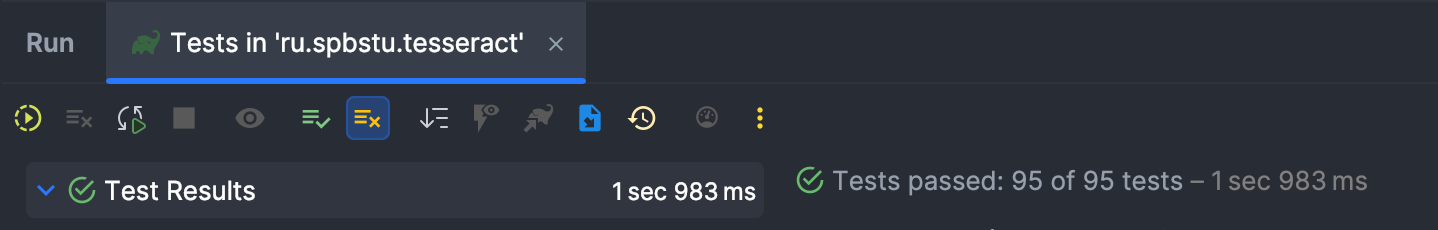
\includegraphics[width=13cm]{resources/2.png}\\
    \caption{Тесты серверной части}
\end{figure}

\begin{figure}[H]
    \centering
    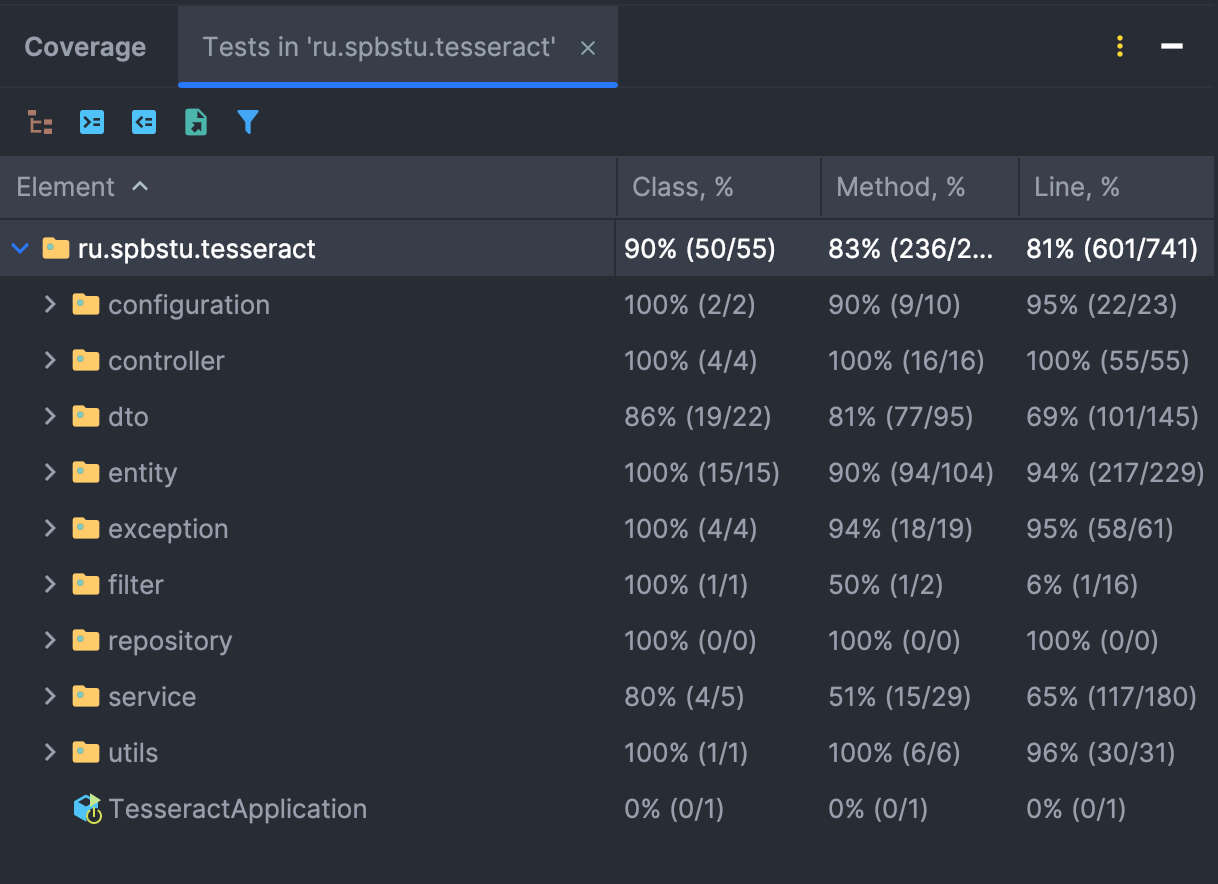
\includegraphics[width=13cm]{resources/3.png}\\
    \caption{Покрытие кода тестами серверной части}
\end{figure}


Для серверной части было написано \textbf{55} тестов, которые покрыли \textbf{91.8\%} кода:

\begin{figure}[H]
    \centering
    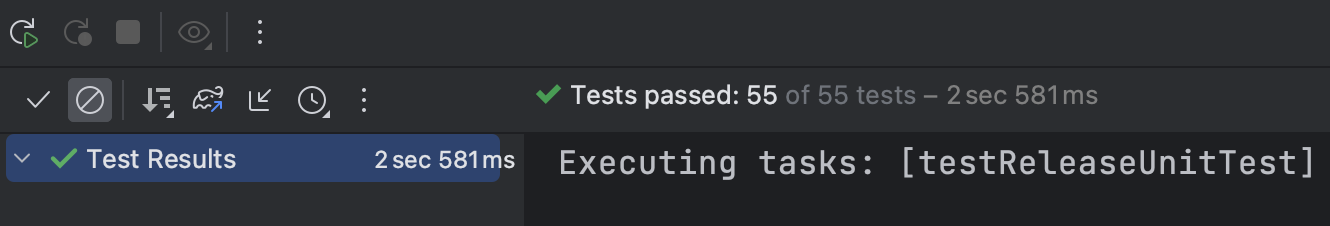
\includegraphics[width=13cm]{resources/4.png}\\
    \caption{Тесты клиентской части}
\end{figure}

\begin{figure}[H]
    \centering
    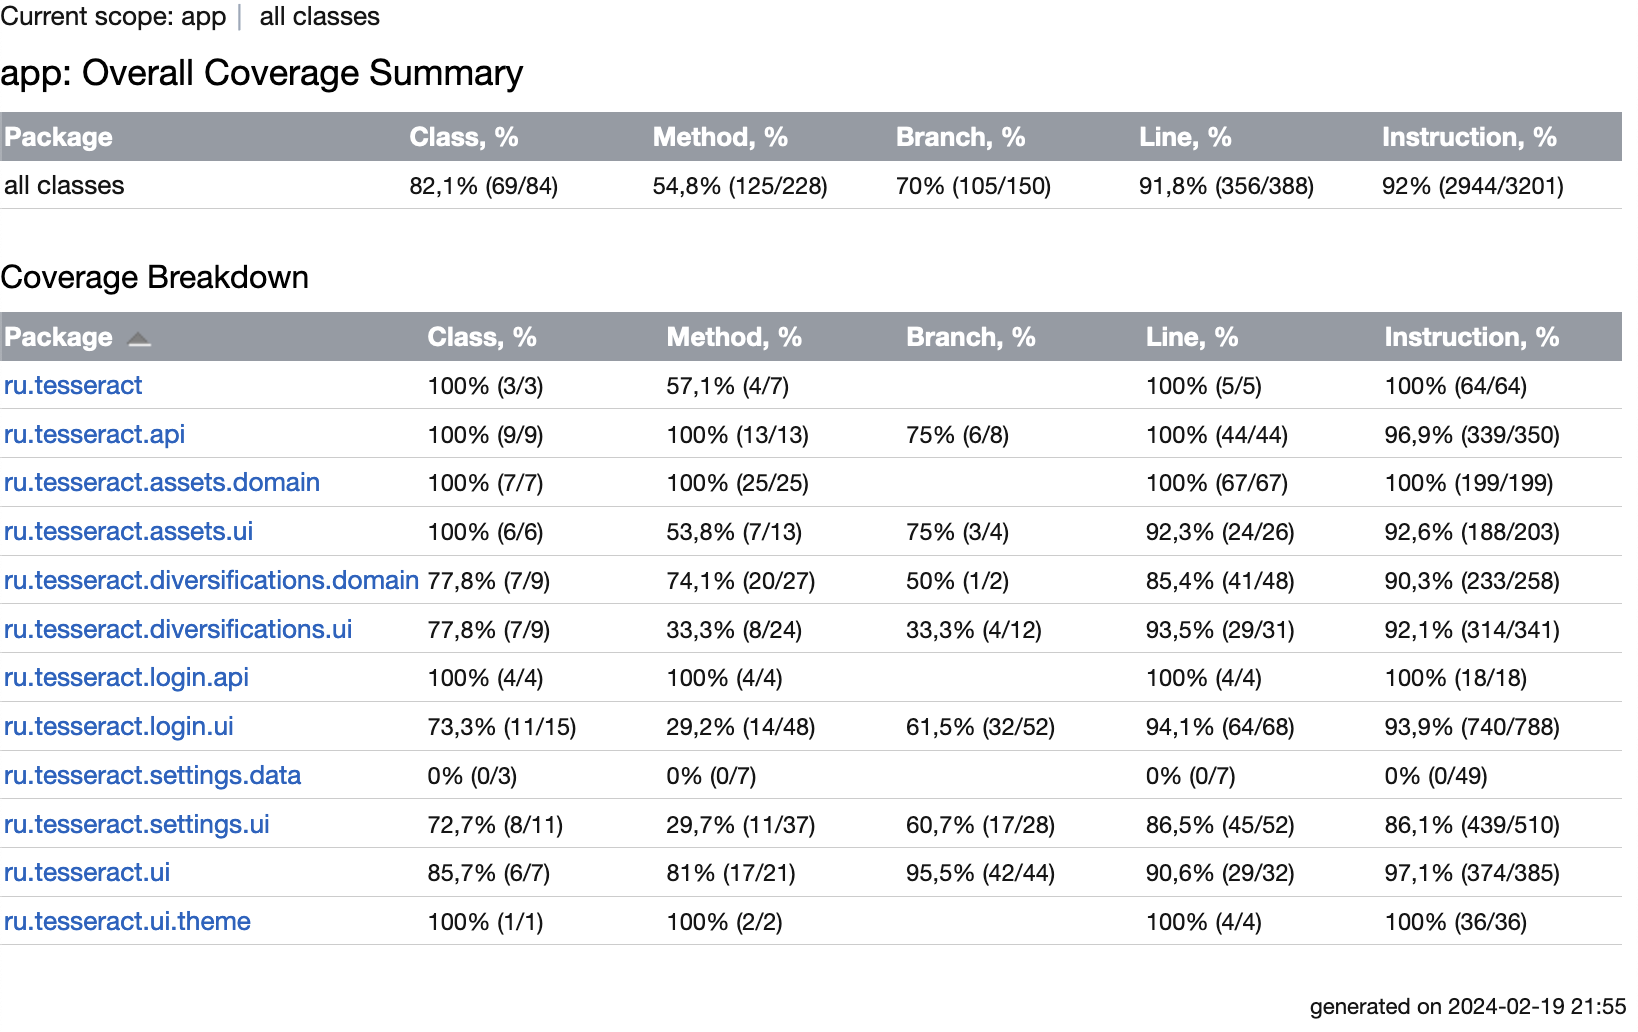
\includegraphics[width=13cm]{resources/5.png}\\
    \caption{Покрытие кода тестами клиентской части}
\end{figure}

\subsection{Описание процедуры расширения тестового набора на примере добавления нового блока, кода, алгоритма, метода}

Для того, чтобы добавить новый тест в код приложения в обоих случаях (клиент, сервер) достаточно в файле, предназначенном для тестов создать функцию, помеченную аннотацией \texttt{@Test} из фреймворка \texttt{JUnit}.

Далее следует выполнить действия, которые составляют суть теста и завершить тест необходимыми проверками.

\end{document}